% Canonical caption for figSendingPoverty.pdf
% Generated by: programs/paper0/sending_poverty.py from the
% aggregates of programs/student_success/linkage_profile.py.
% Regenerate: python programs/paper0/sending_poverty.py
\begin{figure}[tbp]
  \centering
  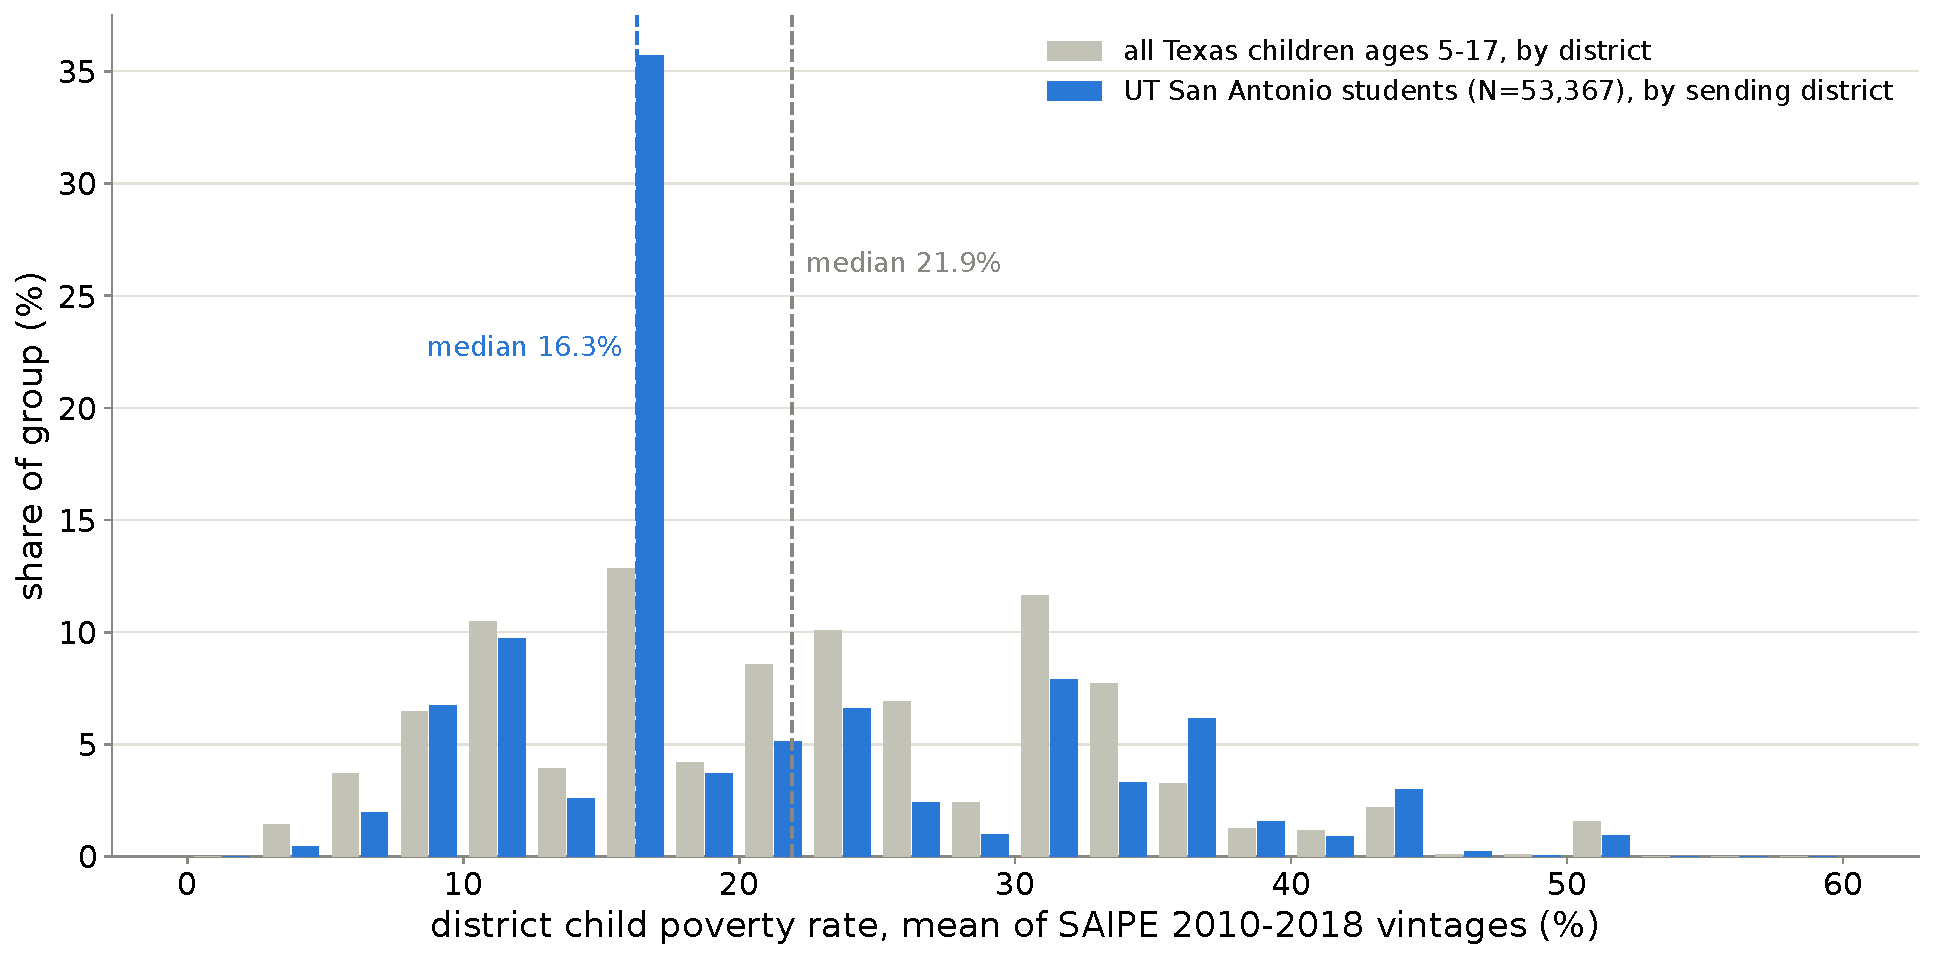
\includegraphics[width=\textwidth]{figSendingPoverty.pdf}
  \caption{Child poverty of the sending districts. Gray: the
    distribution of district child poverty (mean SAIPE rate,
    2010--2018 vintages) over all Texas children aged 5--17,
    weighting each district by the children it holds. Blue: the
    same distribution over the 53,367 students active
    between Fall 2014 and Fall 2019 whose sending high school
    resolves to a Texas public school district
    (682 districts), weighting each district by the
    students it sent. Weights are aggregate counts; no
    student-level record enters the exhibit. Dashed lines mark
    the weighted medians.
    The exhibit reaches 88.9\% of
    the 60,045 students with a Texas high-school name. The
    district poverty of the other students is unobserved, so
    the blue distribution describes the matched students only.}
  \label{figSendingPoverty}
\end{figure}
